\section{\rcc Design}
\label{sec:rcc_overview}

\rcc analyzes both single-router and network-wide properties of BGP
configuration and outputs a list of configuration faults.  \rcc checks
that the BGP configuration satisfies a set of constraints, which are
based on a correctness specification.  Figure~\ref{fig:rcc_arch}
illustrates \rccns's high-level architecture.

We envision that \rcc has three classes of users: 
those that wish to run \rcc with no modifications, 
those that wish to add new constraints concerning the existing
specification, 
and
those that wish to augment the high-level specification.
%Although we believe most network operators have seemed content to run
%\rcc ``out of the box'', 
\rccns's modular design allows users to specify
other constraints without changing the system internals.
Some users may wish to extend the high-level specification to include other
aspects of correctness (\eg, safety~\cite{Griffin2002}) and map those
high-level specifications to constraints on the configuration.

%Designing such a tool presents several challenges.  
%
%First, configuration is complex and distributed across hundreds of
%routers.  Additionally, we must design a way to represent the
%configuration in a format that is amenable to checking constraints.
In this section, we describe how \rcc generates a normalized
representation of the configuration that facilitates constraint
checking.
%
As described in Section~\ref{sec:correct}, we use the correctness
specification from Chapter~\ref{chap:rlogic} as a guide for deriving
actual correctness constraints that \rcc can check against the
normalized configuration.  Section~\ref{sec:mapping} explains this
process.




\begin{figure}[t]
\centering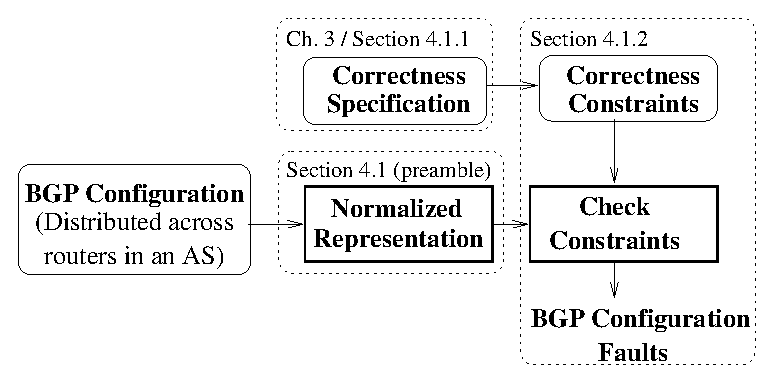
\epsfig{file=rcc/figures/rcc_arch.eps, width=0.9\linewidth}
\caption{Overview of \rccns.}
\label{fig:rcc_arch}
\end{figure}


%\subsection{Generating the Normalized Representation}

%\rcc normalizes BGP configuration to facilitate checking constraints.
\rcc implements the normalized representation as a set of relational
database tables.  This approach allows 
constraints to be expressed independently of router configuration
languages.  As configuration languages evolve and new ones emerge, only
the parser must be modified.  It also
facilitates testing network-wide properties, since all of
the information related to the network's BGP configuration can be
summarized in a handful of tables.  A relational structure is natural
because many sessions share common attributes (\eg, all sessions to the
same neighboring AS often have the same policies), and many policies
have common clauses (\eg, all eBGP sessions may have a filter that is
defined in exactly the same way).  Table~\ref{tab:if} summarizes these
tables; Section~\ref{sec:parser} details how \rcc populates them.

%; a more na\"{i}ve approach would require
%scanning all information about router loopback addresses and session
%information for every iBGP session.

\begin{table}[t]
\centering
%{\footnotesize
\begin{tabular}{lp{5in}}
{\bf Table} & {\bf Description} \\ \hline
%%%%%%%%%%%%%%%%%%%%
%router\_global & 
{\tft global options} & router, various global options (\eg, router ID)\\

%%%%%%%%%%%%%%%%%%%%
%sessions & 
{\tft sessions} & router, neighbor IP address, eBGP/iBGP,
pointers to policy, options (\eg, route-reflector client)\\ 

%%%%%%%%%%%%%%%%%%%%
%networks & 
{\tft prefixes} & router, prefix originated by this router\\

%%%%%%%%%%%%%%%%%%%%
%prefix\_acls & 
{\tft import/export filters} & normalized representation of filter:
IP range, mask range, permit or deny\\ 

%%%%%%%%%%%%%%%%%%%%
%route\_maps & 
{\tft import/export policies} & normalized representation of
policies \\
%; each policy represented by one or more rows
%; each row is a
%clause in the policy \\ 


%%%%%%%%%%%%%%%%%%%%
%router\_loopbacks & 
{\tft loopback address(es)} & router, loopback IP address(es)\\

%%%%%%%%%%%%%%%%%%%%
%router\_interfaces & 
{\tft interfaces} & router, interface IP address(es)\\


%%%%%%%%%%%%%%%%%%%%
%routes & 
{\tft static routes} & static routes for prefixes\\ \hdashline[1pt/1pt]

\multicolumn{2}{c}{{\bf Derived or External Information}} \\

%%%%%%%%%%%%%%%%%%%%
%parse\_errors & 
{\tft undefined references} & policies and filters that a
BGP configuration referenced but did not define\\

%%%%%%%%%%%%%%%%%%%%
%bogon\_list & 
{\tft bogon prefixes} & prefixes that should always be filtered on eBGP
sessions~\protect\cite{www-cymru-bogon}\\ 


%%%%%%%%%%%%%%%%%%%%
%%%%%%%%%%%%%%%%%%%%
%as_regexps & \\
%comm_regexps & \\ 
%communities & & \\ 
%router_sessions & \\
%sessions_shutdown & \\
\end{tabular}
%}
\caption{Normalized configuration representation.}
\label{tab:if}
\end{table}



\subsection{Applying the Correctness Specification to BGP Configuration} 
\label{sec:correct}

\rccns's correctness specification uses the properties from
Chapter~\ref{chap:rlogic} as a starting point. \rcc checks two aspects
of the correctness specification outlined in Chapter~\ref{chap:rlogic}:
{\em path visibility} and \emph{route validity}.  \rcc finds path
visibility and route validity violations in {\em BGP configuration
only}. To make general statements about path visibility and route
validity, \rcc assumes that the internal routing protocol (\ie, interior
gateway protocol, or ``IGP'') used to establish routes between any two
routers within a AS is operating correctly.  BGP requires the IGP to
operate correctly because iBGP sessions may traverse multiple IGP hops
and because the ``next hop'' for iBGP-learned routes is typically
several IGP hops away.

\rcc detects faults that cause {\em persistent} failures.  Both
Chapter~\ref{chap:rlogic} and previous work (\eg,~\cite{Griffin2002})
have studied conditions on the relationships between iBGP and
IGP configuration that must be satisfied to guarantee that iBGP
converges; \rcc does not yet parse IGP configuration, so it does not
check for violations of these constraints.
%
The correctness specifications and constraints assume that,
given stable inputs, the routing protocol {\em eventually} converges to
some steady state behavior.

Currently, \rcc only detects faults in the BGP configuration of a {\em
single AS} (a network operator typically does not have access to the BGP
configuration from other ASes).  Fortunately, because an AS's BGP configuration
explicitly controls both dissemination and filtering, many configuration
faults, including partitions, route leaks, etc., can be detected by
analyzing the BGP configurations of set of the routers in a single AS.


%We define constraints that must be satisfied to guarantee that the
%above properties hold.  For example, when a router imports a route
%from a neighboring AS, validity requires that it should not permit
%routes to prefixes that (1)~originate within its own as or (2)~are
%private or unallocated.  Similarly, when a router advertises a route
%to another router via iBGP, validity requires that the next-hop
%attribute of that route be reachable, and that every route along the
%IGP path to that next hop agree on the same next-hop.  To derive a
%reasonable set of tests, we perform this exercise for both validity
%and visibility for every step of BGP's operation.



%\subsection{Assumptions and Limitations}\label{sec:assumptions}

\subsection{Deriving Correctness Constraints and Detecting
  Faults}\label{sec:mapping} 


\begin{table}[t]
\hspace*{-0.1in}
\begin{center}
{\footnotesize
\begin{tabular}{@{}p{2in}p{3in}@{}}
{\bf Problem} & {\bf Possible Active Fault}\\ \hline \hline
%
\multicolumn{2}{@{}c@{}}{{\it Path Visibility}} \\ \hline
{\bf Dissemination Problems} \\
Signaling partition: & Router may learn a suboptimal route \\
\hspace*{0.1in} - of route reflectors &     or none at all. \\ 
\hspace*{0.1in} - within a RR ``cluster'' \\
\hspace*{0.1in} - in a ``full mesh'' \\

Routers with duplicate: & {Routers may incorrectly drop routes.} \\ 
\hspace*{0.1in} - loopback address \\ 
\hspace*{0.1in} - cluster ID \\

iBGP configured on one end & {Routers won't exchange
routes.} \\  
iBGP not to loopback & {iBGP session fails
when one interface fails.} \\  
%synchronization enabled & \parbox{2in}{iBGP route won't be used if the
%route doesn't also appear in IGP.} \\

\hline \hline
\multicolumn{2}{@{}c@{}}{{\it Route Validity}} \\ \hline
{\bf Filtering Problems} \\
transit between peers & \parbox{4in}{Network carries
traffic ``for free''.} \\
inconsistent export to peer & \parbox{2in}{Violation of contract.} \\
inconsistent import & \parbox{4in}{Possible unintentional
``cold potato'' routing.} \\
%{\bf Undefined References} \\
\parbox{2.18in}{
eBGP session: \\
\hspace*{0.1in} - w/no filters \\ 
\hspace*{0.1in} - w/undef. filter \\
\hspace*{0.1in} - w/undef. policy \\
filter: \\
\hspace*{0.1in} - w/missing prefix \\
policy: \\
\hspace*{0.1in} - w/undef. AS path \\
\hspace*{0.1in} - w/undef. community \\
\hspace*{0.1in} - w/undef. filter \\
}
& \parbox{3in}{
\begin{itemize}
\itemsep=-1pt
\item leaked internal routes
\item re-advertising bogus routes
\item accepting bogus routes from neighbors
\item unintentional transit between peers
\end{itemize}
}
\\
%\hdashline[1pt/1pt]



\hdashline[1pt/1pt]
{\bf Dissemination Problems} \\
prepending with bogus AS & \parbox{4in}{AS path is no longer valid.} \\
originating unroutable dest. & \parbox{4in}{Creates a blackhole.} \\ 
incorrect next-hop & {Other routers may be unable to reach
the routes for a next-hop that is not in the IGP.} \\

\hline\hline
\multicolumn{2}{@{}c@{}}{{\it Determinism}} \\ \hline


{\bf Ranking Problems} \\
\parbox{4in}{nondeterministic MED \\
age-based tiebreaking} 
& \parbox{4in}{Route selection depends on message order.}


\end{tabular}
}
\end{center}

\caption{BGP configuration problems that \rcc detects and their
potentially active faults.} 
\label{tab:rcc_tests}
\end{table}

Deriving constraints on the configuration itself that guarantee that the
correctness specification 
is satisfied is challenging. We reason about how the aspects of
configuration from Section~\ref{sec:semantics} affect each correctness
property and derive appropriate constraints for each of these aspects.
Table~\ref{tab:rcc_tests} summarizes the correctness
constraints that 
\rcc checks, which follow from determining which aspects of
configuration affect each aspect of the
correctness specification (from Section~\ref{sec:correct}).
These constraints are an attempt to map the path visibility and route
validity specifications to constraints on BGP configuration that can be
checked against the actual configuration.  


%Path visibility constraints typically address
%potential problems with how iBGP routes propagate through the AS, or
%``iBGP signaling'' (Section~\ref{sec:visibility}).  \rccns's route
%validity constraints test 
%potential problems with policy configuration or how routes are
%advertised (Section~\ref{sec:validity}).  
%The ``miscellaneous''
%constraints can affect both
%path visibility and route validity.
Ideally, operators would run \rcc to detect configuration faults {\em
before} they are deployed.  Some of \rccns's constraints detect faults
that would most likely become active immediately upon deployment.  For
example, a router that is advertising
routes with an incorrect next-hop attribute will immediately prevent
other routers that  
use those routes from forwarding packets to those
destinations.  In this case, \rcc can help a network operator diagnose
configuration faults and prevent them from introducing failures on the
live network.  
%Many constraints in Table~\ref{tab:rcc_tests} detect {\em
%latent} faults, detection of latent faults is very important because the
%operator may not unaware of an erroneous configuration until some input
%actually triggers the fault (at which time the failure can be quite
%serious).  

Many of the constraints in Table~\ref{tab:rcc_tests} concern faults that
could remain undetected even after the configuration has been deployed
because they remain masked until some sequence of messages triggers
them. In these cases, \rcc can help operators find faults that could
result in a serious failure.  Section~\ref{sec:visibility} describes one
such path visibility fault involving dissemination in iBGP in further
detail. 
%For example, an operator will likely not notice that a BGP
%session to a neighboring AS applies an undefined filter until that
%neighbor ``leaks'' an invalid route.  
%
In other cases, checking constraints implies some knowledge of high-level
policy (recall that route validity, as defined in
Definition~\ref{defn:rv}, concerns a path that conforms to some 
high-level policy).  In the absence of a high-level policy specification
language, 
\rcc must make inferences about a network operator's intentions.
Section~\ref{sec:validity} describes several route validity faults where
\rcc must make such inferences.


%\rcc checks the constraints against the normalized representation of the
%BGP configuration.  Section~\ref{sec:visibility} describes how \rcc uses
%the BGP session-level topology to detect path visibility faults in iBGP.
%Section~\ref{sec:validity} explains how \rcc uses beliefs and closures
%to detect route validity faults.  Section~\ref{sec:verifier} describes
%how \rcc checks these constraints in practice.


%\subsection{\rccl Architecture}\label{sec:design}



%% Describe architecture of the tool.  How we parse IOS/JunOS into an
%% intermediate format.  Describe the intermediate format, how we organize
%% checks in terms of mysql queries, etc. Three phases: 1. preparsing,
%% 2. parsing, 3. checking


%This section describes the high-level architecture of \rccns.  We
%present the design of \rccns's {\em intermediate configuration format},
%a vendor-independent representation of a network's BGP configuration.
%We then briefly describe the correctness tests that \rcc performs,
%noting how the intermediate configuration format facilitates many of
%these tests.



%\subsection{Verifying the Configuration}


%The intermediate format concisely represents configuration semantics and
%allows an operator to see the entire configuration at a glance.  The
%format implicitly specifies a model of network-wide routing
%configuration.  

%% We decided that the intermediate format should not make
%% any assumptions about how the network structure; rather, the
%% intermediate format should be a general, literal interpretation of the
%% configuration, and the queries against the intermediate format should
%% determine the semantics of the intermediate format.
%% %Accordingly, we had to decide
%% %whether the intermediate format should incorporate strict assumptions
%% %about the network configuration, or whether the format should be general
%% %enough to accept configurations that might not necessarily conform to
%% %the data model:
%% %
%% %\begin{itemize}
%% %\itemsep=-1pt
%% %\item What assumptions about network structure should be built into the
%% %intermediate format?  Should the format impose constraints on the
%% %configuration? 
%% %\end{itemize}
%% On one hand, incorporating strict assumptions about network structure
%% makes certain types of verification tests easier because the
%% intermediate format is guaranteed to conform to the strict model.
%% However, it also means that unorthodox configurations may not conform to
%% the model.  Adopting a more general structure allows unusual
%% configurations to be represented in the intermediate format, but it can
%% verification more difficult because the semantics of the intermediate
%% format are less explicit.

%% For example, the table of BGP sessions contains a column for a
%% ``remote AS''.  A remote AS is typically a unique number and represents a
%% distinct administrative domain, but, in certain cases,
%% the same remote AS may actually connect to {\em different} neighboring
%% networks: an ISP may assign the same AS number to multiple customers if
%% those customers have no other upstream providers.  
%% %In this case, the ISP
%% %should remove the ``customer'' AS number from the AS path before
%% %re-advertising the route.  
%% A single administrative domain
%% may also comprise multiple ASes~\cite{rfc-confederations}.

%% A strict data model might impose a one-to-one mapping between an AS and
%% an administrative domain, which would make certain
%% correctness tests easier: \rcc would know that all private AS numbers
%% should be removed on sessions to remote ASes, and, when comparing
%% policies across multiple sessions to the same AS number, it could know
%% that those policies were being applied to the same neighboring network.  
%% A more general data model would accept the configuration information,
%% even if the configuration was not sensible, and rely on the
%% verification process to report possible problems.  This approach
%% may cause the verifier to generate false positives: for example, the
%% verifier may wrongly report that a private AS should be removed from the
%% AS path of an ``eBGP'' session, when, in fact, the ``eBGP'' session is
%% a session to a router with a different AS number in the same
%% administrative domain.

%% Because BGP configuration is flexible, it is difficult to design a
%% strict format that will accept all sensible
%% configurations.  (In Section~\ref{sec:evaluation}, we will describe many
%% anomalies that \rcc discovered that illustrate that BGP can be
%% configured in many different ways to achieve the same task.)  We decided
%% that the
%% intermediate format should serve as a literal representation of the
%% configuration, without applying any sanity checks.  This decision has
%% worked well in practice: the fact that \rcc can load any configuration
%% into the intermediate format (rather than rejecting a configuration
%% because it does not fit the data model) allows it to be considerably
%% more usable.  Although this approach generates more false positives,
%% distinguishing more serious errors from ``anomalies'' has proved to be
%% relatively easy in practice.


%\subsection{Checking the Constraints}
%\label{s:verification}


\subsection{Completeness and Soundness}


\begin{figure}[t]
\centering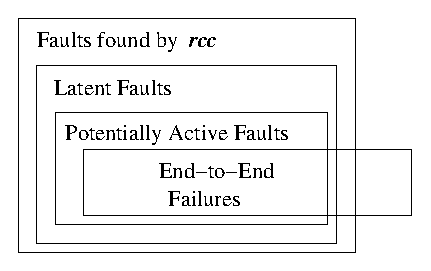
\epsfig{file=rcc/figures/faults2.eps, width=0.6\linewidth}
\caption{Relationships between faults and failures.}
\label{fig:faults}
\end{figure}

%% caveats and setting the fence
%\rccns's constraints are neither complete (\ie,
%they may not find all problematic configurations) nor sound (\ie, they
%may report problems that are simply deviations from best common
%practice), but static analysis techniques for program analysis
%are typically neither complete nor sound either~\cite{Musuvathi2003}.
%As discussed in Section~\ref{sec:mapping}, \rcc is neither complete nor
%sound.  
\rccns's constraints are neither complete nor sound; that is, they may
not find all problematic configurations, and they may complain about
harmless deviations from best common practice.  However, practical
static analysis techniques for program analysis are typically neither
complete nor sound, either~\cite{Musuvathi2003}.
Figure~\ref{fig:faults} shows the relationships between classes
of configuration faults and the class of faults that \rcc detects.  {\em
Latent faults} are faults that are not actively causing any problems but
nonetheless violate the correctness constraints.  A subset of latent
faults are {\em potentially active} faults, for which there is at least
one input sequence that is certain to trigger the fault.  For example,
an import policy that references an undefined filter on a BGP session to
a neighboring AS is a potentially active fault, which will be triggered
when that neighboring AS advertises a route that ought to have been
filtered.  When deployed, a potentially active fault will become {\em
active} if the corresponding input sequence occurs.  An active fault
constitutes a routing failure for that AS.

Some active faults may ultimately appear as {\em end-to-end failures}.
For example, if an AS advertises an invalid route (\eg, a route for a
prefix that it does not own) to a neighboring AS whose import policy
references an undefined filter, then some end hosts may not be able to
reach destinations within that prefix.  Note that a 
potentially active fault may not always result in an end-to-end failure
if no path between the sources and destinations traverses the routers in
the faulty AS.  

\rcc detects a subset of latent (and hence,
potentially active) faults.  In addition, \rcc
may also report some false positives: faults that violate the
constraints but are {\em benign} (\ie, the violations 
would never cause a failure).
Ideally, \rcc would detect fewer benign faults 
by testing the BGP configuration against an abstract specification.
Unfortunately,
producing such a specification requires additional work from
operators, and operators may well write incorrect specifications.  
One of \rccns's advantages is that it provides useful information about
configuration faults without requiring any additional work on the part
of operators.


Our previous work~\cite{Feamster2003b} presented three properties in
addition to path visibility and route validity: information flow control
(this property checks if routes ``leak'' in violation of policy),
determinism (whether a router's preference for routes depends on the
presence or absence of other routes), and safety (whether the protocol
converges)~\cite{Griffin2002c}.  Our definitions of route validity
(Definition~\ref{defn:rv}),
policy (Definition~\ref{defn:policy}), and policy-conformant paths
(Definition~\ref{defn:pcp}) incorporate the notion of information flow
control.  With a couple of exceptions (see Table~\ref{tab:rcc_tests}),
\rcc does not check for faults related
to determinism and safety.  Many aspects of determinism depend on the
route selection process that are inherent in today's practices (\eg, the
fact that MED is only comparable across routes received from the same
neighboring AS) and cannot be effectively checked using static analysis.
Safety is a property of the global routing system that, in practice,
requires access to configurations from multiple ASes to check.  In
Chapter~\ref{chap:policy}, we derive constraints that guarantee safety
with access to configurations of only a single AS and find that these
conditions are quite restrictive.


%\subsubsection{Intermediate Format Overview}








%%%%%%%%%%%%%%%%%%%%%%%%%%%%%%%%%%%%%%%%%%%%%%%%%%%%%%%%%%%%%%%%%%%%%%
%Since the intermediate format is simply a set of relational
%database tables, \rcc can check each correctness constraint by
%executing one ore more SQL queries against the database containing the
%configuration state.


%\footnote{We implemented all
%  correctness checks from 
%Section~\ref{sec:analysis} except those from previous
%work~\cite{Griffin2002}, which require knowledge about shortest
%IGP paths through the network, but, due to space constraints, we
%describe only two checks here: one ``single router'' check, and one that
%requires testing properties of the graph.}  

%Certain 
%queries involve comparing the entries from two tables. For example,
%\rcc checks whether every route that is originated by BGP has a
%corresponding route; this requires comparing entries in the {\tf
%networks} table against those from the {\tf routes} table.


%However, \rccns's extensible design
%facilitates adding these checks.

%% (might allude here to simple checks vs. complex checks)  not really
%% going to discuss pattern-based vs. whatever anymore.  simple checks
%% reall just entail checking bit-flips.  complex can involve multiple
%% routers, interaction with IGP, etc.

%% Also discuss the need to know default settings sometimes.  That is, even
%% the simple ``bit flip'' checks have subtleties.  For example, the avici
%% (and procket) story, where ``no sync'' is enabled by default.  An ideal
%% version of the checker should keep track of routing vendor, OS version
%% numbers, etc., and a detailed list of what's enabled/disabled by default
%% for a particular router.



%%\subsection{\rccl Intermediate Configuration Format}\label{sec:if}









%Note that we do {\em not}
%assume that BGP converges: its steady state for a fixed input
%might be oscillatory.


%\subsubsection{Challenges}\label{sec:challenges}

%BGP configuration errors are difficult to detect because they often
%appear far from the actual source of the error and may not appear
%immediately after the deployment of an erroneous configuration.
%(Sections~\ref{sec:validity} and~\ref{sec:visibility} discuss at greater
%length configuration errors that are not immediately apparent.)  As a
%result, operators must often search for errors in a trial-and-error
%fashion.

%\rcc performs both ``basic'' single-router configuration checks and more
%complicated network-wide checks.  We discovered that even syntactic
%errors on a single router often fail silently: in one network, \rcc
%found a session that applied an undefined filter that would have allowed
%that AS's customer to advertise any prefix.  These types of errors are
%relatively easy to find because they only involve looking at single
%configuration files in isolation.
%%\footnote{Previous work
%% single-router checks that do not specifically address
%%the correctness of any particular protocol~\cite{FeldmannXXXX}; we
%%perform similar checks for BGP and extend
%%this work in several ways: 
%%(1)~we report statistics on the errors we have found in practice; (2)~we
%%have made our tool publicly available to network operators; and (3)~our
%%tool is in use by many ISPs.}.  
%Analyzing the {\em network-wide} behavior of BGP configuration, on the
%other hand, requires synthesizing configuration across all of the
%routers in the AS, which presents several challenges:
%\begin{CompactEnumerate}

%\item {\em BGP configuration is distributed.}  Verifying BGP
%  configuration requires checking dependencies across multiple routers.
%  For example, determining how (and whether) routes propagate between
%  routers requires parsing the configurations of every router in the
%  network to construct an {\em session-level graph} of iBGP sessions, as well
%  as determining how policies are applied on each of those sessions (and
%  how the policies relate to one another).

%\item {\em BGP configuration is network-specific.}  BGP
%  configuration is flexible enough to allow network operators to
%  implement the same behavior in many different ways.  In fact, an
%  operator may implement the {\em same} policy in several different ways
%  on routers in the same AS.  \rcc must {\em canonicalize} BGP
%  configuration by representing it in some normalized format.

%\item {\em BGP configuration is vendor-specific.}  Any single AS may may
%  use routers from several different router vendors: nearly every
%  network we analyzed used at least two router vendors, and one small
%  ISP we analyzed used routers from four different vendors.  To analyze
%  these networks, \rcc must be able to represent BGP configuration in
%  some {\em vendor-independent} format.  In practice, designing such a
%  format is tricky: Vendor configuration languages have vastly different
%  syntax and even have slight differences in semantics.  For example, in
%  Cisco IOS, the next-hop attribute is assigned as a session-level
%  option, whereas in JunOS, the next-hop is assigned in policy statements.

%\end{CompactEnumerate}

%To address these challenges, we represent the network-wide set of
%configuration files as a collection of database tables.  This
%normalized format allows \rcc to quickly access information about
%groups of BGP sessions or policies and makes the verification process
%independent from configuration syntax and specifics.  We describe the
%normalized format in more detail in Section~\ref{sec:parsing}.


%% We address these challenges by viewing BGP as a distributed program,
%% rather than a protocol that conforms to a set specification.\footnote{We
%% explain in Section~\ref{s:related} why the absence of a 
%% specification makes verifying wide-area routing using
%% approaches like model checking infeasible.}  We determine a set of
%% invariants that 
%% should hold true independent of the details of configuration.  Many of
%% these invariants are verifiable using static analysis.
%% %
%% We also determine which invariants require checking configurations at a
%% single router and which require checks across multiple routers.
%% Fortunately, we find that many serious problems can be uncovered with
%% checks that only require configurations from routers {\em within a
%% single network}.
%\footnote{Griffin and Wilfong's ``safety'' violation
%caused by incompatible policies in different networks is an
%exception~\cite{Griffin2002c}; see Section~\ref{s:safety}.}  

%% \item {\em Defining ``correctness'' is difficult.}  Operators configure BGP
%% to achieve a variety of tasks.  Defining
%% ``correctness'' for a protocol that can behave in many ways is
%% difficult.  We use the {\em routing logic}~\cite{Feamster2003b} to help
%% us define correctness properties and constraints.



%\rcc performs static analysis on a set of BGP configurations from
%routers in a single AS and outputs a list of faults.
%Figure~\ref{fig:rcc_arch} illustrates this approach.  
%Section~\ref{sec:correct} defines a specification for two aspects of
%routing correctness---path visibility and
%route validity.
%\rcc normalizes
%vendor-specific router configurations into an normalized
%format (Section~\ref{sec:parsing}),
%analyzes the normalized format
%(Section~\ref{s:verification}), and produces a list of faults.



%In
%fact, we believe that it is highly unlikely that network operators would
%have paid attention to \rcc had it not been software that works ``out of
%the box'' on existing configurations without requiring any other
%operator input.


%\rcc detects faults by testing a set of
%constraints on BGP configuration based on the correctness specification
%we propose in Section~\ref{sec:correct} and outlined in more detail in
%Section~\ref{s:verification}.  These faults may be latent 
%(some of these are potentially active), but \rcc may also find {\em
%benign} (\ie, false positives).  \rcc is also not guaranteed to catch
%all latent faults.  



%%% Set the fence here

%
%A {\em potentially active fault} is a latent fault for 
%A latent fault is a {\em potentially active fault} if it may
%cause BGP to violate correctness, but may require a particular execution
%path to
%actually cause a violation.  
%



%% Why is this task challenging?
%% Analyzing BGP routing is akin to analyzing a distributed program,
%% because most (if not all) faults that occur in practice are caused by
%% statements in router configurations.  Because BGP configuration is
%% distributed, analyzing the network-wide behavior of a set of routers
%% requires the ``joint analysis'' of their configurations and an
%% assessment of the interactions and dependencies between them.
%% Additionally, configuration languages are flexible: the same high-level
%% routing behavior (\eg, a particular policy) can be implemented in
%% multiple ways on a given set of routers.  In addition, each router
%% vendor has a different configuration language, and these languages are
%% not entirely feature-compatible.  \rcc addresses these challenges by
%% using a vendor-independent normalized configuration format based on
%% the relational data model.

%% move to related work
%Other tools perform some
%single-router consistency checks that catch fundamental
%mistakes~\cite{Caldwell2003}, 
%%but verifying BGP correctness requires
%%analyzing a {\em network-wide} view of configuration and a {\em
%%definition of correctness}.  \rcc executes network-wide correctness
%%checks based on a high-level definition of correctness.


%We believe that one reason that
%\rcc has enjoyed a relatively high level of acceptance is because it
%works ``out of the box'': it provides useful information to network
%operators while requiring no additional effort on their part.


%\subsection{Approach}

%Figure~\ref{fig:rcc_arch} illustrates the \rccns's high-level approach
%to BGP configuration checking.  \rcc expects a set of router
%configurations from a single AS, which can be collected from the routers
%using existing tools such as ``rancid''~\cite{www-rancid}.  Ultimately,
%\rcc outputs information that helps operators track down BGP
%configuration errors.  To do this, \rcc must first have a set of
%properties to check;  describes our high-level
%approach for describing these checks.  Because \rcc attempts to make
%statements about a single protocol using only the configurations, it
%must make some assumptions, which we describe in
%Section~\ref{sec:assumptions}.  Section~\ref{sec:challenges} explains
%why checking properties of distributed router is
%difficult in practice.
